In this section, we compare STRUCT to a state-of-the-art NLG system,
CRISP~\footnote{We considered using the PCRISP system as a
  baseline~\cite{bauer_sentence_2010}. However, we could not get the system to
  compile, and we did not receive a response to our queries, so we were
  unable to use it.}
and evaluate three hypotheses: (i) STRUCT is
comparable in speed and generation quality to CRISP as it generates
increasingly large referring expressions, (ii) STRUCT is
comparable in speed and generation quality to CRISP as the size of the
grammar which they use increases, and (iii) STRUCT is capable of
communicating complex propositions, including multiple concurrent
goals, negated goals, and nested subclauses.
Finally, we evaluate the effect on STRUCT's performance 
of varying key parameters, including grammar size.

We compare CRISP to two different versions of STRUCT.
As mentioned in the previous chapter, there are two different reward
functions which we have written and found to be useful in this
domain.  We compare to both such functions in order to demonstrate
the performance tradeoffs of a system based on a reward function.
STRUCT was implemented in Python 2.7, where CRISP was implemented
in Java.  All of our experiments were run on a 4-core AMD Phenom II X4 995 processor
clocked at 3.2 GHz.  Both systems were given access to 8 GB of RAM.

\section{Comparison to CRISP}

We begin by describing experiments comparing STRUCT to CRISP. We used a
2010 version of CRISP  which uses a Java-based GraphPlan
implementation. In these
experiments, we use a deterministic grammar.
Because the reward signal is fine-grained,
 a myopic action selection strategy is
sufficient for these experiments, and 
the $d$ parameter is set to zero. The
number of simulations for STRUCT varies between 20 to 150.
In most cases, a small $n$, under 100, is sufficient
to guarantee generation success.  The exploration constant $c$ in
Equation~\ref{eqn:uct} is irrelevant when $n$ is less than the size
of the set of actions, since it
applies only to actions selected after all open actions have already
been tried once.

\begin{figure}
\centering
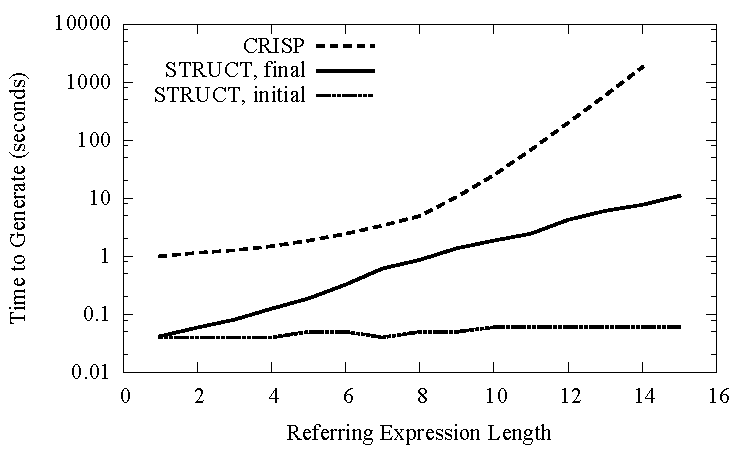
\includegraphics[width=0.7 \linewidth ]{../analysis/plots/complex-goal/complex-goal.pdf}
\caption{Experimental comparison between STRUCT and  CRISP: 
Generation time vs. length of referring expression }
\label{crisp-comparison-gentime}
\end{figure}

\begin{figure}
\centering
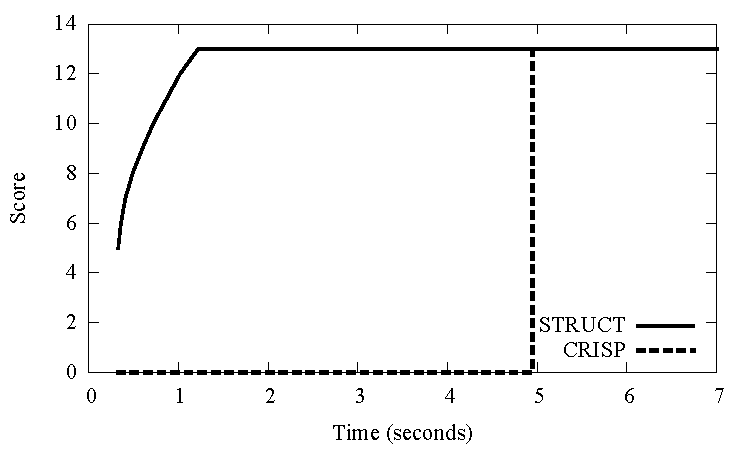
\includegraphics[width=0.7 \linewidth ]{../analysis/plots/complex-goal/complex-goal-anytime.pdf}
\caption{Experimental comparison between STRUCT and  CRISP:
Score of best solution vs time.}
\label{crisp-comparison-score}
\end{figure}

\subsection{Referring Expressions}
We first evaluate CRISP and STRUCT on their ability to generate
referring expressions. We follow prior work (\cite{koller_experiences_2011})
in our initial experiment design.  We consider a series of sentence
generation problems which require the planner to generate a sentence
like ``The Adj$_1$ Adj$_2$ ... Adj$_k$ dog chased the cat.",
where the string of adjectives is a string that distinguishes one
dog (whose identity is specified in the problem description) from
all other entities in the world.
The experiment has two parameters: $j$, the number of adjectives in
the grammar, and $k$, the number of adjectives necessary to
distinguish the entity in question from all other entities. We set $j
= k$ and show the results in Figure~\ref{crisp-comparison-gentime}.
We observe that CRISP was able to achieve
sub-second or similar times for all expressions of less than length 5, but its
generation times increase exponentially past that point, exceeding 100
seconds for some plans at length 10. At length 15, CRISP failed to
generate a referring expression; after 90 minutes the Java garbage
collector terminated the process. STRUCT$_b$, performs much better and
is able to generate much longer referring expressions without failing.
Later experiments had successful referring expression generation of lengths
as high as 25.  STRUCT$_a$ performs similarly to CRISP asymptotically.

We can also observe the anytime nature of STRUCT from this experiment,
shown in Figure~\ref{crisp-comparison-score}.  Here we look at the
length of the solution sentence generated as a function of time, for
$k=8$, a mid-range scenario which both generators are able to solve
relatively quickly ($< 5s$).  As expected, CRISP produces nothing until
the end of its run, at which point it returns the solution. STRUCT (both versions)
quickly produces a reasonable solution, ``The dog chased the
cat.''  This is then improved upon by adjoining until the referring
expression is unambiguous. If at any point the generation process was
interrupted, STRUCT would be able to return a solution that at least
partially solves the communicative goal.

In this experiment, $d$ was set equal to 1, since each action taken improved the sentence in
a way measurable by our reward function.  $n$ was set equal to $k * (k + 1)$, since this is
the number of adjoining sites available in the final step of generation, times the number
of potential words to adjoin.  This allows us to ensure successful generation in a single
loop of the STRUCT algorithm.

\begin{figure}
\centering
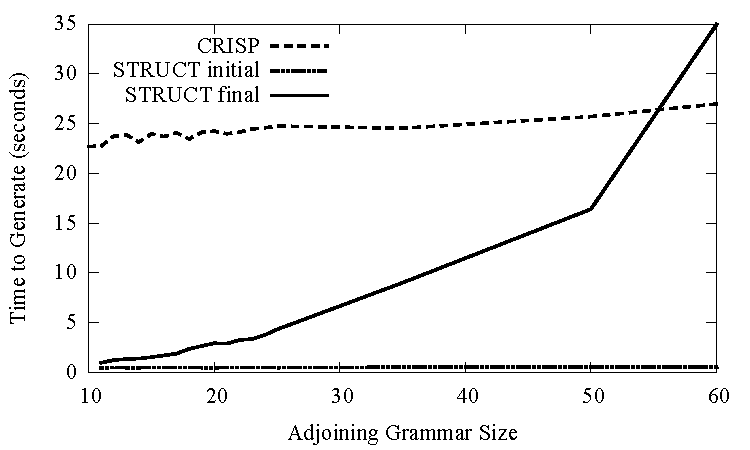
\includegraphics[width=0.7 \linewidth]{../analysis/plots/large-grammar/large-grammar.pdf}
\label{graph-large-grammars}
\caption{Effect of grammar size}
\end{figure}

\begin{figure}
\centering
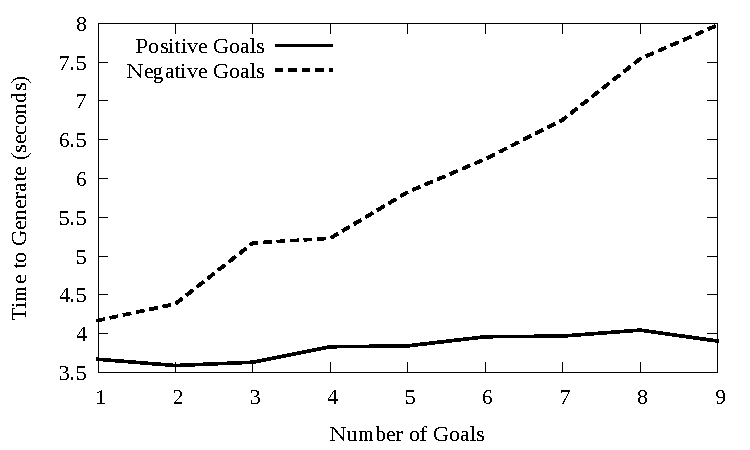
\includegraphics[width=0.7 \linewidth]{../analysis/plots/goals/differentgoals.pdf}
\label{chart-different-goals}
\caption{Effect of multiple and negated goals}
\end{figure}

\subsection{Grammar Size}
We next evaluate STRUCT and CRISP's ability to
handle larger grammars. This experiment is set up in the same way as
the one above, with the exception of $l$ ``distracting'' words, words
which are not useful in the sentence to be generated.  $l$ is defined
as $j - k$.  In these experiments, we vary $l$ between 0 and 50.
Figure~\ref{graph-large-grammars} shows the results of these
experiments.  We observe that CRISP using GraphPlan, as previously
reported in \cite{koller_experiences_2011}, handles an increase in
number of unused actions very well.  Prior work reported a difference
on the order of single milliseconds moving from $j = 1$ to $j = 10$.
We report similar variations in CRISP runtime as $j$ increases from 10
to 60: runtime increases by approximately 10\% over that range.

\subsubsection{Absent Pruning}

STRUCT's performance with large grammars is similar to CRISP using the
FF planner \cite{hoffmann_ff_2001}, also profiled in
\cite{koller_experiences_2011}, which increased from 27 ms to 4.4
seconds over the interval from $j = 1$ to $j = 10$.  STRUCT's
performance is less sensitive to larger grammars than this, but over
the same interval where CRISP increases from 22 seconds of runtime to
27 seconds of runtime, STRUCT increases from 4 seconds to 32 seconds.
This is due almost entirely to the required increase in the value of
$n$ (number of samples) as the grammar size increases.  At the low
end, we can use $n=20$, but at $l = 50$, we must use $n = 160$ in
order to ensure perfect generation as soon as possible.  Fortunately,
as STRUCT is an anytime algorithm, valid sentences are available very
early in the generation process, despite the size of the set of
adjoining trees (the ``STRUCT Initial'' curve in
Figure~\ref{graph-large-grammars}).  This value does not change
substantially with increases in grammar size.  However, the time to
improve this solution does.

\subsubsection{With Pruning}

STRUCT's performance with large grammars improves dramatically if
we allow for pruning (described in Chapter 4).  This experiment involving distracting words
is a perfect example of a case where pruning will perform well.
When we apply pruning we find that STRUCT is able to completely ignore the effect of
additional distracting words.  Experiments showed roughly constant times for generation
for $j=1$ through $j=5000$.  Although pruning is $O(n)$ in grammar size, repeated experiments
failed to show any significant distinction in runtime, even on very large grammars.

\section{Evaluation of Complex Communicative Goals}
In the next set of experiments, we illustrate that STRUCT can solve
conjunctions of communicative goals as well as negated communicative goals.

\subsection{Multiple Goals}
We next evaluate STRUCT's ability to accomplish
multiple communicative goals when generating a single sentence.  In this
experiment, we modify the problem from the 
previous section.  In that section, the referred-to dog was unique,
and it was therefore possible to produce a referring expression which
identified it unambiguously.  In this experiment, we remove this
condition by creating a situation in which the generator will be
forced to ambiguously refer to several dogs.  We then add to the
world a number of adjectives which are common to each of these
possible referents.  Since these adjectives do not further
disambiguate their subject, our generator should not use
them in its output.  We then encode these adjectives into
communicative goals, so that they will be included in the output of
the generator despite not assisting in the accomplishment of
disambiguation.  For example, assume we had two black cats, and
we wanted to say that one of them was sleeping, but we wanted
to emphasize that it was a black cat.  We would have as our goal
both ``sleeps(c)" and ``black(c)".  We want the generator to
say ``the black cat sleeps", instead of simply ``the cat sleeps".

We find that, universally, these otherwise useless
adjectives are included in the output of our generator, demonstrating
that STRUCT is successfully balancing multiple communicative goals.
As we show in figure \ref{chart-different-goals} (the ``Positive
Goals'' curve) , the presence of additional satisfiable semantic goals does
not substantially affect the time required for generation.  We are able to
accomplish this task with the same very high frequency as the CRISP
comparisons, as we use the same parameters.

\subsection{Negated Goals}
We now evaluate STRUCT's ability to generate
sentences given negated communicative goals.  We again modify
the problem used earlier by 
adding to our lexicon several new adjectives, each applicable only to
the target of our referring expression.  Since our target can now be
referred to unambiguously using only one adjective, our generator
should just select one of these new adjectives (this has been experimentally confirmed).
We then encode these
adjectives into negated communicative goals, so that they will not be
included in the output of the generator, despite allowing a much
shorter referring expression.  For example, assume we have a
tall spotted black cat, a tall solid-colored white cat, and a short spotted
brown cat, but we wanted to refer to the first one without
using the word ``black".

We find that these adjectives which
should have been selected immediately are omitted from the output, and
that the sentence generated is the best possible under the
constraints.  This demonstrates that STRUCT is balancing these negated
communicative goals with its positive goals.  Figure
\ref{chart-different-goals} (the ``Negative Goals'' curve) shows the
impact of negated goals on the time to generation.  Since this
experiment alters the grammar size, we see the time to final
generation growing linearly with grammar size.  The increased time to
generate can be traced directly to this increase in grammar size.
This is a case where pruning does not help us in reducing the grammar size;
we cannot optimistically prune out words that we do not plan to use.  Doing
so might reduce the ability of STRUCT to produce a sentence which partially
fulfills its goals.

\subsection{Nested subclauses}

\begin{figure}
\centering
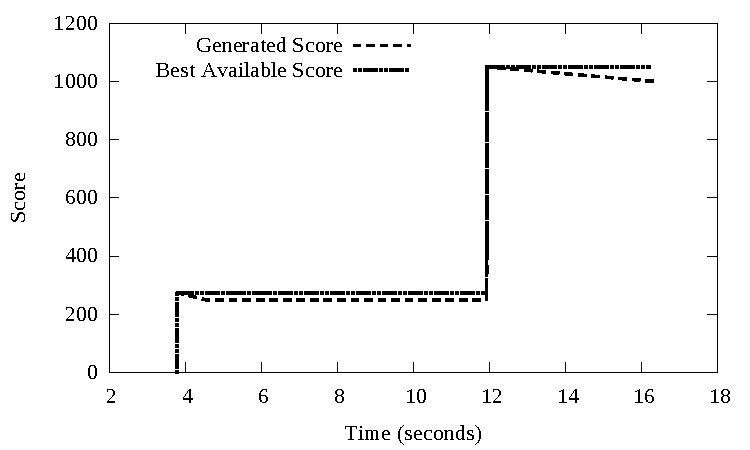
\includegraphics[width=0.7\linewidth]{../analysis/struct/nested/nested.pdf}
\caption{Reward function output over time as STRUCT generates a sentence with a nested subclause}
\label{nested}
\end{figure}

Here, we evaluate STRUCT$_a$'s ability to generate sentences with nested
subclauses.  An example of such a sentence is ``The dog which ate the treat
chased the cat".  This is a difficult sentence to generate for several reasons.
The first, and clearest, is that there are words in the sentence which do not
help to increase the score assigned to the partial sentence.  Notably, we must adjoin
the word "which" to "the dog" during the portion of generation where the
sentence reads "the dog chased the cat".  This decision requires us to do planning
deeper than one level in the MDP, which increases by $O(N^d)$ the number of simulations
STRUCT requires in order to get the best possible result.

Despite this issue, STRUCT is capable of generating these sentences.  As we can
see in Figure \ref{nested}, STRUCT's time to generate increases with the number of
nested clauses.  To the best of our knowledge, CRISP is not able to generate sentences
of this form due to an insufficiency in the way it handles TAGs,
and consequently we present our results without baselines.  We present
results only for STRUCT$_a$ here, since STRUCT$_b$ is not capable of generating
sentences using indirection.

In this case, we require lookahead further into the tree than depth 1.  We need to know
that using ``which" will allow us to further specify which dog is chasing the cat;
in order to do this we must use at least $d=3$.  Our reward function will determine this
with, at a minimum, the actions corresponding to ``which", ``ate", and ``treat".

\subsection{Conjunctions}

\begin{figure}
\centering
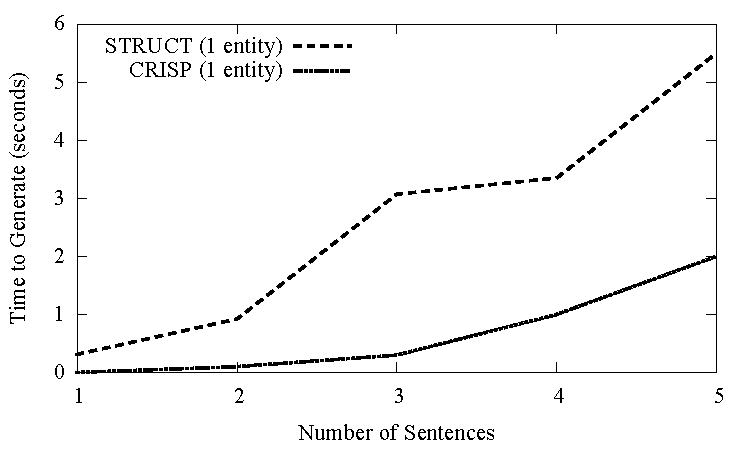
\includegraphics[width=0.7 \linewidth]{../analysis/struct/conjunction/conjunction1.pdf}
\label{graph-conjunction1}
\caption{Time to generate sentences with conjunctions with one entity ("The man sat and the girl sat and ....").
Note that STRUCT performs slightly worse than CRISP with one entity.}
\end{figure}

\begin{figure}
\centering
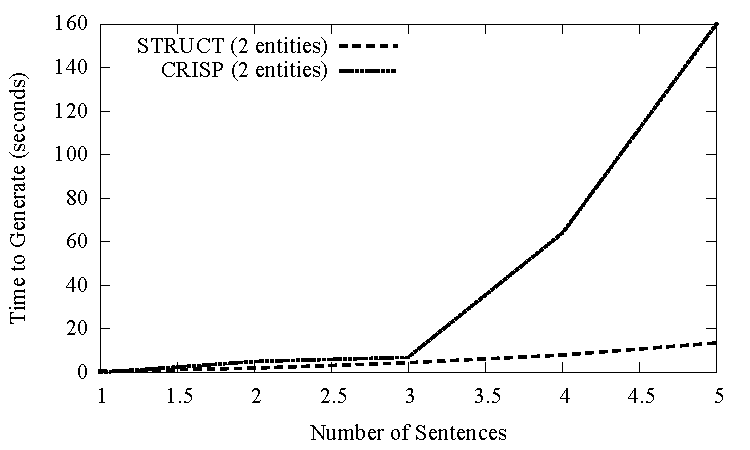
\includegraphics[width=0.7 \linewidth]{../analysis/struct/conjunction/conjunction2.pdf}
\label{graph-conjunction2}
\caption{Time to generate sentences with conjunctions with two entities ("The dog chased the cat and ...").  Note that
STRUCT performs much better than CRISP with two entities.}
\end{figure}

\begin{figure}
\centering
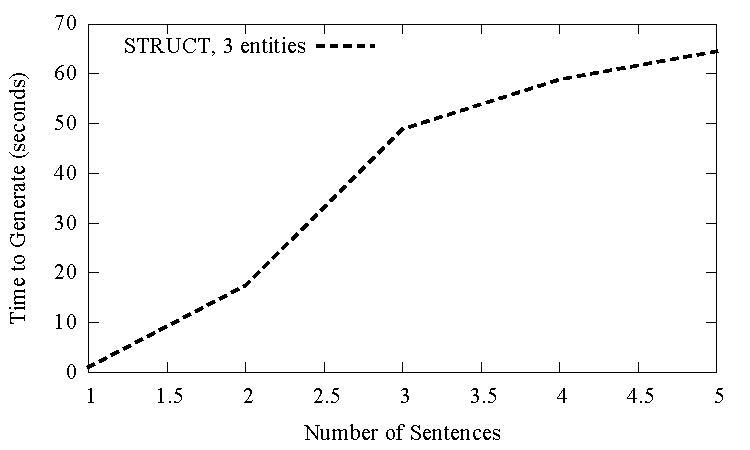
\includegraphics[width=0.7 \linewidth]{../analysis/struct/conjunction/conjunction3.pdf}
\label{graph-conjunction3}
\caption{Time to generate sentences with conjunctions with three entities ("The man gave the girl the book and ....").
CRISP cannot generate sentences with conjunctions and three entities; STRUCT is much less sensitive to a change
in the number of entities than CRISP.}
\end{figure}

Here, we evaluate STRUCT$_b$'s ability to generate sentences including
conjunctions.  We introduce the conjunction "and", which allows for the
root nonterminal of a new sentence ('S') to be adjoined to any other sentence.
We then provide STRUCT with multiple goals.  Given sufficient depth for the
search ($d=3$ was determined to be sufficient, as our reward signal is fine-grained),
STRUCT will produce two sentences joined by the conjunction "and".
Here, we follow prior work in our experiment design \cite{koller_experiences_2011}.

As we can see in Figures \ref{graph-conjunction1}, \ref{graph-conjunction2}, and
\ref{graph-conjunction3}, STRUCT successfully generates results
for conjunctions of up to five sentences.  This is not a hard upper bound, but
generation times begin to be impractically large at that point.
Fortunately, human language tends toward
shorter discourse units than these unwieldy (but technically grammatical) sentences.

STRUCT increases in generation time both as the number of sentences increases and as
the number of objects per sentences increases.  We show results for STRUCT$_a$ here,
as our output should contain only simple sentences without nesting, and because
STRUCT$_b$ is exponential in number of entities in the sentence, which will cause
impractically large generation times for this experiment.

We also compare our results to those presented in \cite{koller_experiences_2011} for
CRISP with the FF Planner.  Koller et al attempted to generate sentences with
three entities and failed to find a result within their 4 GB memory limit.  As we
can see, CRISP generates a result slightly faster than STRUCT when we are 
working with a single entity, but works much much slower for two entities
and cannot generate results for a third entity.  According to Koller's findings,
this is because the search space grows by a factor of the universe size with
the addition of another entity \cite{koller_experiences_2011}.

\section{Summary}

In summary, we have implemented the STRUCT algorithm in Python 2.7 and tested
it in a variety of situations, including several which are difficult for CRISP and which
challenge our generator's ability to prune, to generate complex referring expressions,
to generate nested clauses, and to generate long and very complex sentences.
In all these cases, STRUCT was able to accomplish the communicative
goals without trouble, in a reasonable amount of time.  We found that, in general,
STRUCT's asymptotic behavior is comparable to CRISP's, but in the region
where most language generation takes place, STRUCT performs approximately as well
or better.

We have also shown that STRUCT is capable of generating language that CRISP simply
cannot (referring expression), and that STRUCT is capable of anytime generation.
These properties make STRUCT a desirable natural language generator, even
compared to the state-of-the-art generator we used.